\justy{Poniżej prezentujemy 6 diagramów klas klienta i 6 diagramów klas serwera.}

\subsubsection{Diagramy klas klienta}
\begin{figure}[H]
	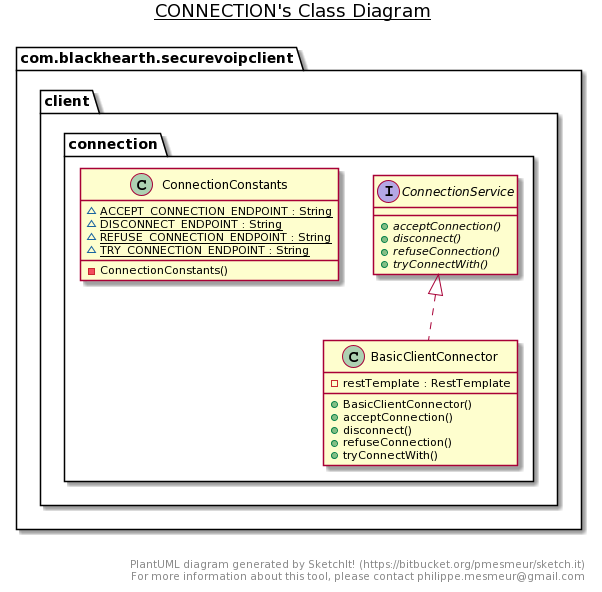
\includegraphics[width=0.5\textwidth]{images/uml/1.png}
	\centering	
	\caption{\centering Diagram klas serwisu łączącego dwóch klientów.}
\end{figure}
\begin{figure}[H]
	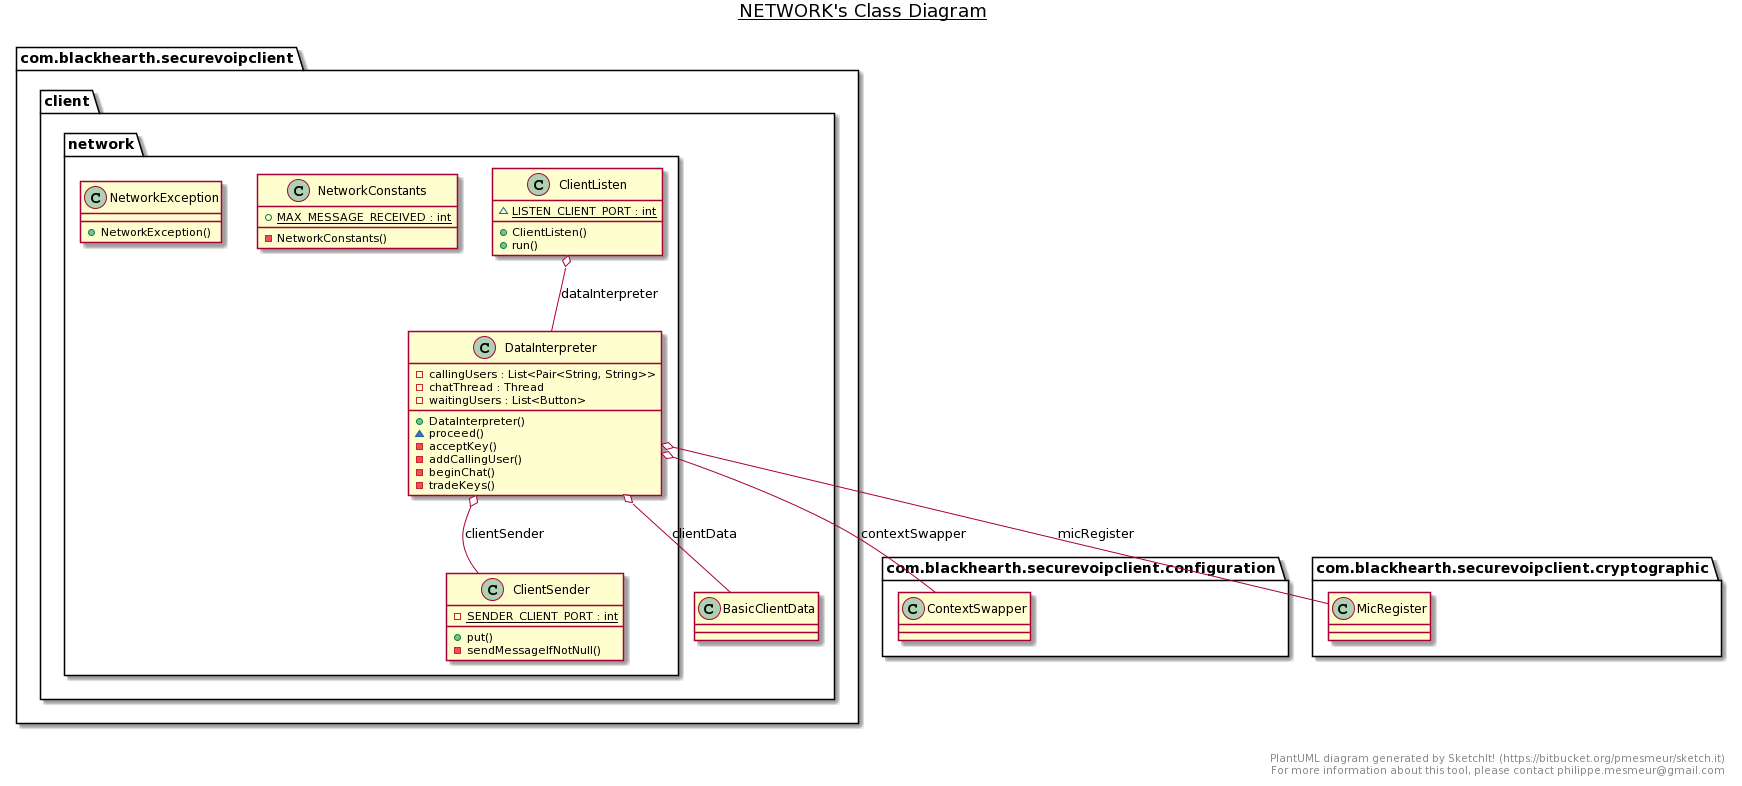
\includegraphics[width=0.5\textwidth]{images/uml/2.png}
	\centering	
	\caption{\centering Diagram klas połączenia UDP pomiędzy dwoma klientami.}
\end{figure}
\begin{figure}[H]
	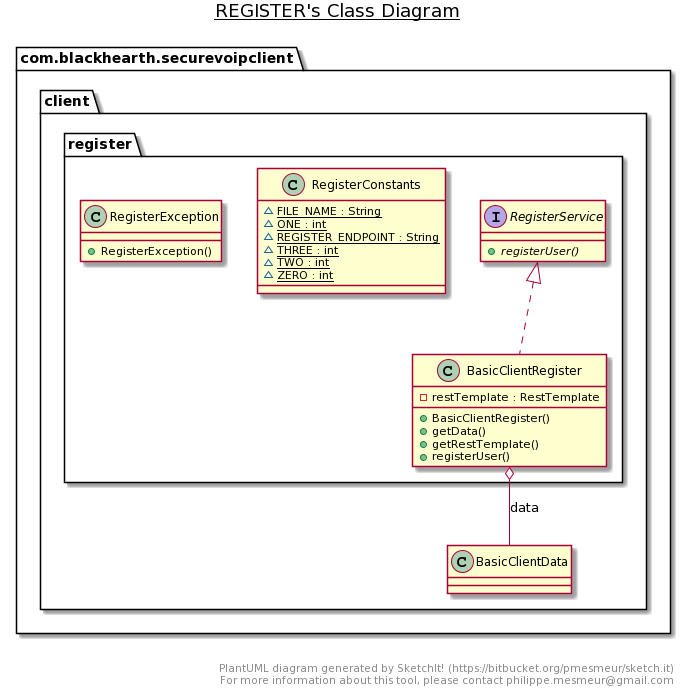
\includegraphics[width=0.5\textwidth]{images/uml/3.png}
	\centering	
	\caption{\centering Diagram klas sewrisu rejestrującego nowego użytkownika.}
\end{figure}
\begin{figure}[H]
	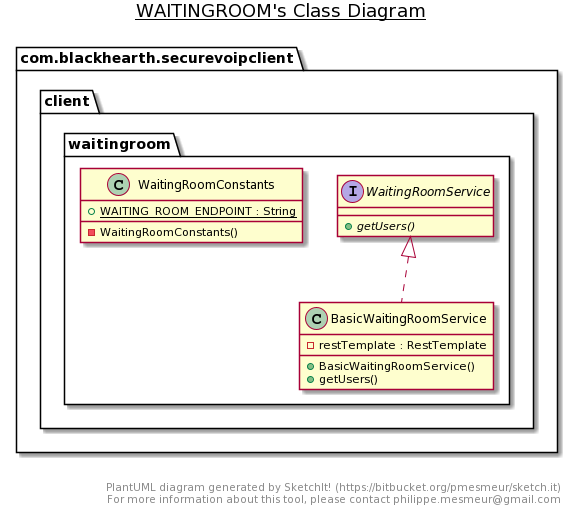
\includegraphics[width=0.5\textwidth]{images/uml/4.png}
	\centering	
	\caption{\centering Diagram klas serwisu pobierającego listę użytkowników z serwera.}
\end{figure}
\begin{figure}[H]
	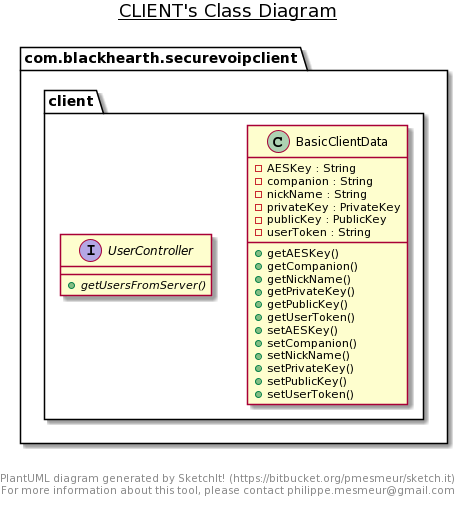
\includegraphics[width=0.5\textwidth]{images/uml/5.png}
	\centering	
	\caption{\centering Diagram klas danych użytkownika.}
\end{figure}
\begin{figure}[H]
	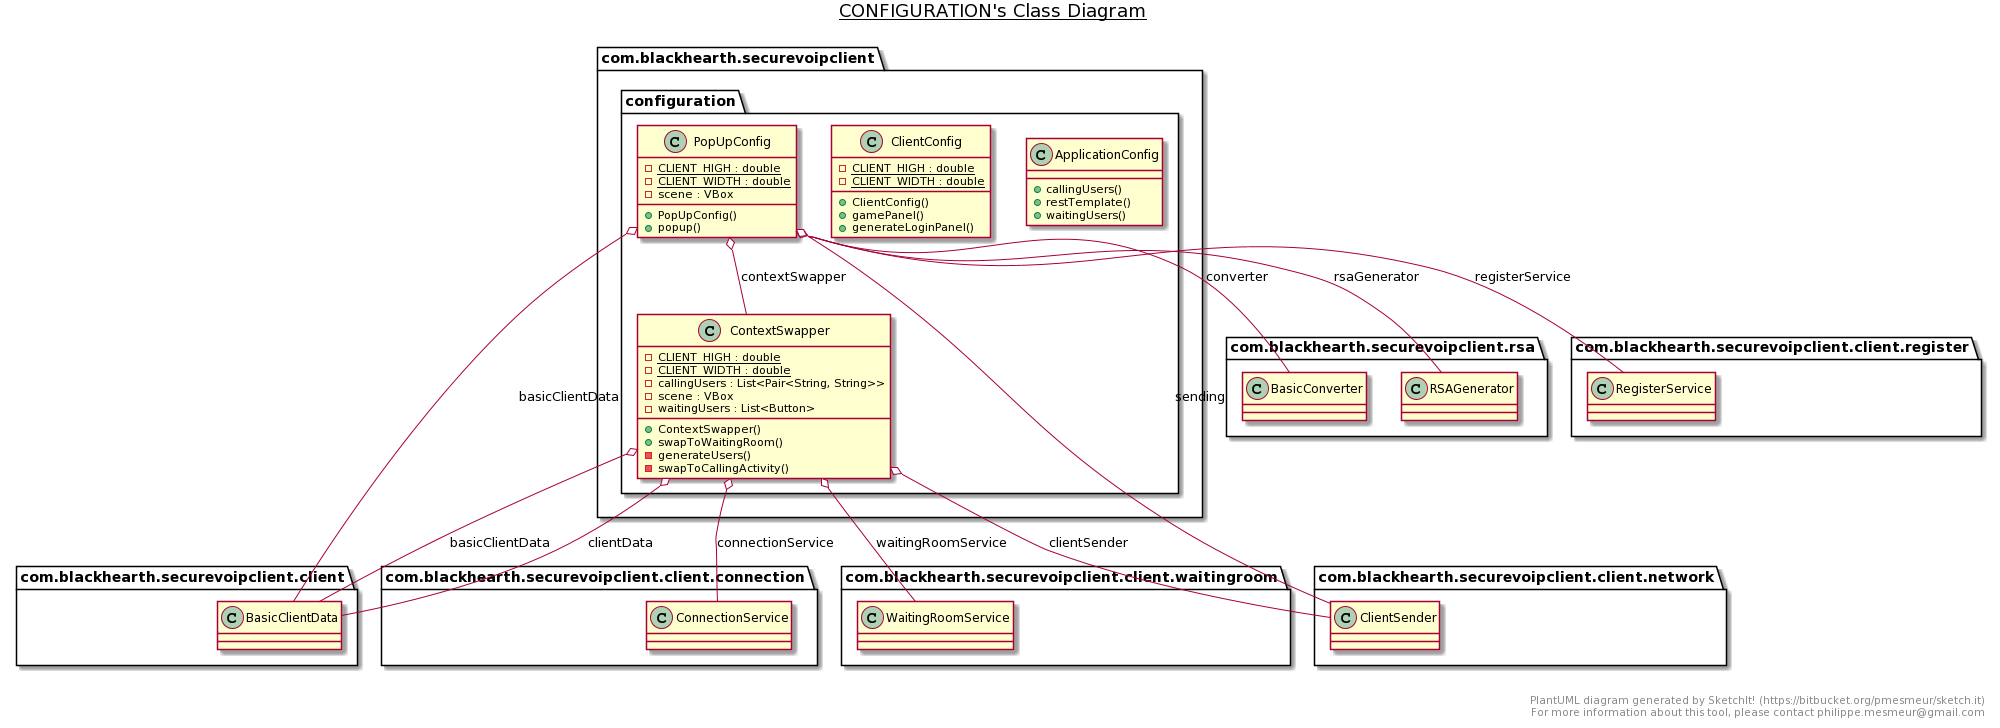
\includegraphics[width=0.5\textwidth]{images/uml/6.png}
	\centering	
	\caption{\centering Diagram klas konfiguracji klienta.}
\end{figure}

\subsubsection{Diagramy klas serwera}
\begin{figure}[H]
	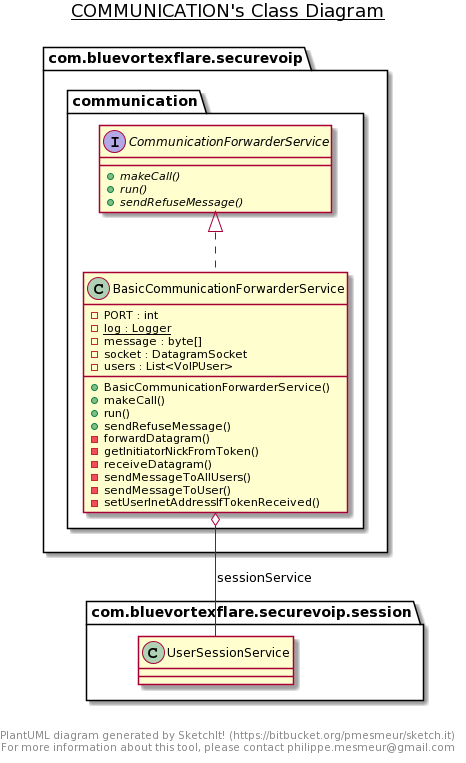
\includegraphics[width=0.5\textwidth]{images/uml/s1.png}
	\centering	
	\caption{\centering Diagram klas połączenia UDP pomiędzy serwerem a klientem.}
\end{figure}
\begin{figure}[H]
	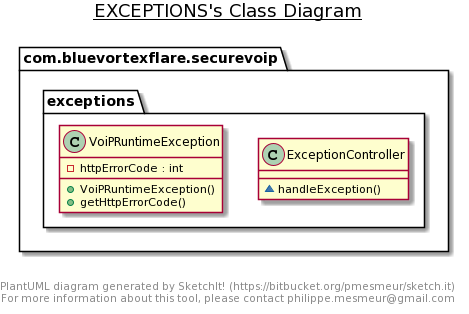
\includegraphics[width=0.5\textwidth]{images/uml/s2.png}
	\centering	
	\caption{\centering Diagram klas wyjątków serwera.}
\end{figure}
\begin{figure}[H]
	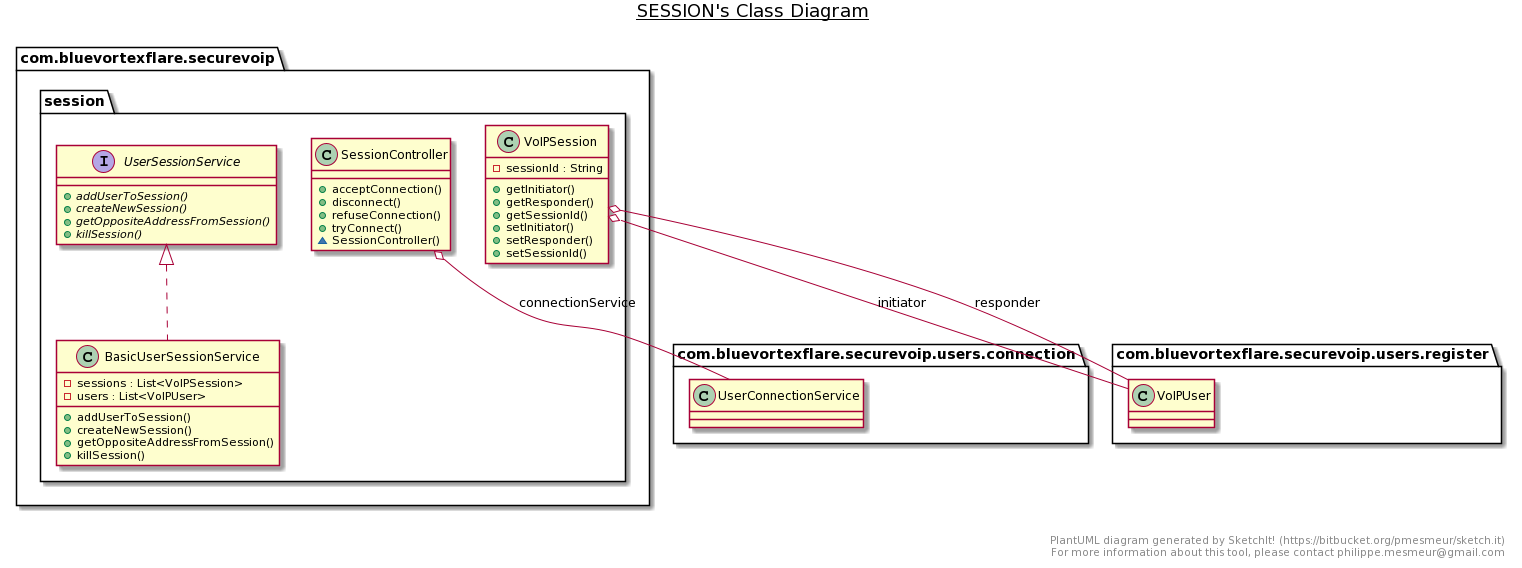
\includegraphics[width=0.5\textwidth]{images/uml/s3.png}
	\centering	
	\caption{\centering Diagram klas serwisu zarządzającego sesjami użytkowników.}
\end{figure}
\begin{figure}[H]
	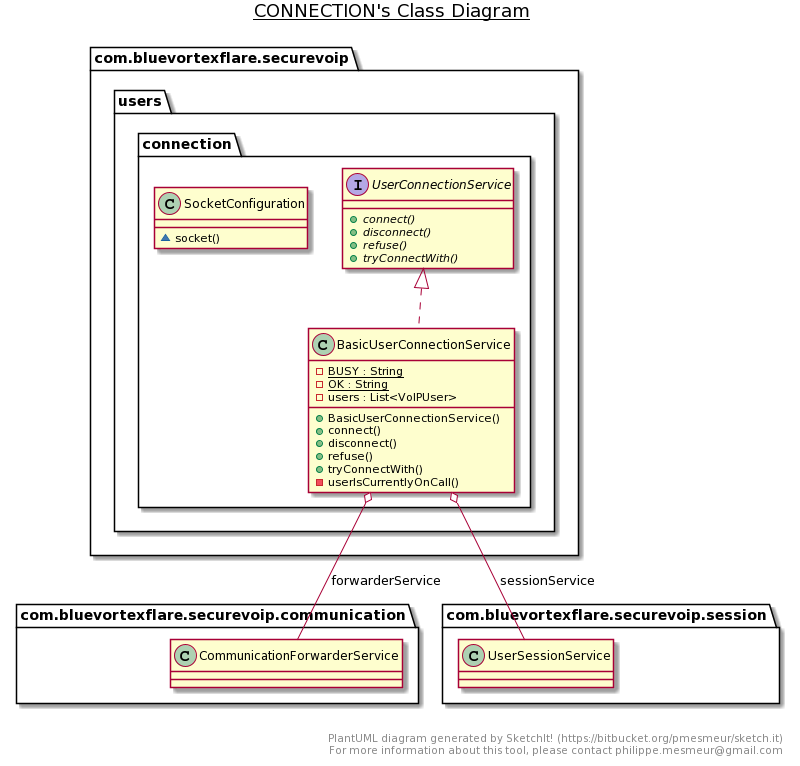
\includegraphics[width=0.5\textwidth]{images/uml/s4.png}
	\centering	
	\caption{\centering Diagram klas serwisu zarządzającego połączeniem pomiędzy użykownikami.}
\end{figure}
\begin{figure}[H]
	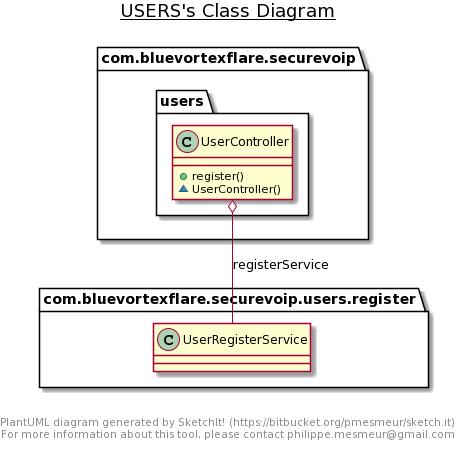
\includegraphics[width=0.5\textwidth]{images/uml/s5.png}
	\centering	
	\caption{\centering Diagram klas ilustrujący zależność pomiędzy kontrolerem użytkownika, a serwisem rejestrującym.}
\end{figure}
\begin{figure}[H]
	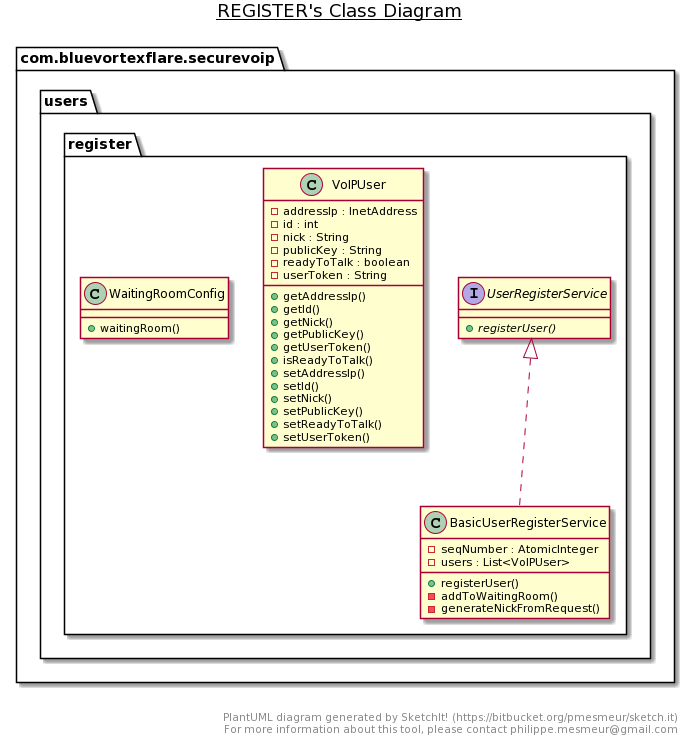
\includegraphics[width=0.5\textwidth]{images/uml/s6.png}
	\centering	
	\caption{\centering Diagram klas serwisu rejestrującego.}
\end{figure}